\documentclass[10pt,letterpaper]{article}
\usepackage[top=1in,bottom=1in,left=1in,right=1in]{geometry}
\usepackage{datetime}
\usepackage{natbib}      % http://merkel.zoneo.net/Latex/natbib.php
\usepackage{palatino}
\usepackage{verbatim}
\usepackage[normalem]{ulem}
\bibpunct{(}{)}{;}{a}{,}{,}

\usepackage{array}

\usepackage{chngpage}
\usepackage{stmaryrd}
\usepackage{amssymb}
\usepackage{amsmath}
\usepackage{graphicx}
\usepackage{lscape}
\usepackage{subfigure}
\usepackage[usenames,dvipsnames]{color}
\definecolor{myblue}{rgb}{0,0.1,0.6}
\definecolor{mygreen}{rgb}{0,0.3,0.1}
\usepackage[colorlinks=true,linkcolor=black,citecolor=mygreen,urlcolor=myblue]{hyperref}

\newcommand{\bocomment}[1]{\textcolor{Bittersweet}{BO says: #1}}

\newcommand{\ignore}[1]{}
\newcommand{\transpose}{^\mathsf{T}}
\newcommand{\inner}[1]{\langle #1 \rangle} 
\newcommand{\smallsec}[1]{\noindent \textbf{#1\ }}
\newcommand{\cmd}[1] {{\color{blue}\texttt{#1}}}

\newcommand{\solution}[1]{{\color{myblue} \emph{[Solution:} 

#1 

\emph{End solution]}}}
\newcommand{\solutionnote}[1]{{\color{myblue} \emph{[Note:}

#1 

\emph{End note]}}}
\newcommand{\points}[1]{{\color{mygreen}\emph{[#1]\ \ }}}

\newcommand{\aone}{\diamondsuit}
\newcommand{\atwo}{\heartsuit}
\newcommand{\bone}{\triangle}
\newcommand{\btwo}{\Box}
\newcommand{\myand}{\ \land\ }
\newcommand{\myor}{\ \lor\ }
\newcommand{\mynot}{\lnot}

\title{
  Homework 1 \\
  \Large{CMPSCI 370 Spring 2018, UMass Amherst} \\
  \Large{Due: February 15, 11:59 PM} \\
  \Large{Instructor: Subhransu Maji} \\
  \Large{TA: Matheus Gadelha}
}

\settimeformat{ampmtime}
\date{}
\begin{document}
\maketitle

\renewcommand\thesubsection{\thesection.\alph{subsection}}


\section*{Guidelines}

\paragraph{Submission.} Submit a \emph{zip file} via moodle that includes a pdf with your solutions and source code. You have a total of 3 late days for all your homework assignments. Delay by even one minute counts as a full late day. Submissions beyond the late days will not be given \emph{any} credit.

\paragraph{Plagiarism.} We might reuse problem set questions from previous years, covered by papers and webpages, we expect the students not to copy, refer to, or look at the solutions in preparing their answers. We expect students to want to learn and not google for answers. Any instance of cheating will lead to zero credit for the homework, and possibly a failure grade for the entire course.

\paragraph{Collaboration.} The homework must be done individually, except where otherwise noted in the assignments. 'Individually' means each student must hand in their own answers, and each student must write their own code in the programming part of the assignment. It is acceptable, however, for students to collaborate in figuring out answers and helping each other solve the problems. We will be assuming that you will be taking the responsibility to make sure you personally understand the solution to any work arising from such a collaboration.

\paragraph{Using other programming languages.} We made the starter code available in Python and Matlab. You are free to use other languages such as Octave or Julia with the caveat that we won't be able to answer or debug non Matlab/Python questions.

\paragraph{Python requirements.} We will be using Python 2.7. The Python starter code requires \cmd{scipy} for loading images and \cmd{numpy} for matrix operations (at least v1.12).
If you are not familiar with installing those libraries through some package manager (like \cmd{pip}), the easiest way of using them is installing \href{https://conda.io/docs/user-guide/install/index.html}{Anaconda}.
%
%\newpage
%\section{Linear algebra review [0 points]}
%We will review some basic concepts in linear algebra relevant to this homework. Linear algebra is the math of vectors and matrices. Let $n$ be a positive integer and let $\mathbb{R}$ denote the set of real numbers, then $\mathbb{R}^n$ is the set of all
%$n$-tuples (an ordered list of size $n$) of real numbers. A vector $\vec{v} \in \mathbb{R}^n$
%is an $n$-tuple of real numbers. For example, consider a vector that has two components: $\vec{v} = (v_1, v_2) \in (\mathbb{R}, \mathbb{R}) \in \mathbb{R}^2$.
%
%A matrix $A \in \mathbb{R}^{m \times n}$ is a rectangular array of real numbers with $m$ rows and $n$ columns. For example, a $2 \times 3$ matrix looks like this:
%
%\[ A = \left[ \begin{array}{ccc}
%a_{11} & a_{12} & a_{13} \\
%a_{11} & a_{12} & a_{13} \end{array} \right] 
%\in 
%\left[
%\begin{array}{ccc}
%\mathbb{R} & \mathbb{R} & \mathbb{R} \\
%\mathbb{R} & \mathbb{R} & \mathbb{R} \end{array} \right]
%\in 
%\mathbb{R}^{3\times 2}
%\]
%\subsection{Vector operations}
%Given vectors $\vec{u} = (u_1, u_2, \ldots, u_n) $ and $\vec{v} = (v_1, v_2, \ldots, v_n) \in \mathbb{R}^n$ we can define various vector operations:
%\begin{itemize}
%\item Addition: $\vec{u} + \vec{v} = (u_1 + v_1, u_2 + v_2, \ldots, u_n + v_n)$
%\item Subtraction: $\vec{u} - \vec{v} = (u_1 - v_1, u_2 - v_2, \ldots, u_n - v_n)$
%\item Dot product: $\vec{u} \cdot \vec{v} = u_1 v_1 + u_2 v_2 + \ldots + u_n v_n$
%\item Length of a vector: $||\vec{u}|| = \sqrt{u_1^2 + u_2^2+\ldots+u_n^2}$. The $||.||$ notation is also called the ``norm".
%\item Distance between two vectors: $d(\vec{u}, \vec{v}) = ||\vec{u}-\vec{v}|| =  \sqrt{(u_1-v_1)^2 + (u_2-v_2)^2+\ldots+ (u_n-v_n)^2}$
%\item Relationship between dot product and distance: $||\vec{u}-\vec{v}||^2 = ||\vec{u}||^2 + ||\vec{v}||^2 - 2\vec{u}\cdot \vec{v}$. You can verify this using the definitions above and the identity $(a-b)^2 = a^2 + b^2 - 2ab$.
%\end{itemize}
%
%Assume that $\vec{u}, \vec{v}$ are of unit length, i.e. $||\vec{u}||=||\vec{v}||=1$. The relationship between the dot product and distance can be simplified in this case to $||\vec{u}-\vec{v}||^2 = 1 + 1 - 2\vec{u}\cdot \vec{v} = 2(1-\vec{u}\cdot \vec{v})$. Thus if the distance between the two vectors is small the dot product is close to $1$, and if the distance is large then the dot product is close to zero. Hence, the dot product can be seen as a \emph{similarity measure}. In fact the dot product normalized by the norm of the vectors measures the cosine of the angle $\theta$ between them, i.e., $\cos \theta = \frac{\vec{u}\cdot \vec{v}}{||\vec{u}||||\vec{v}||}$.
%
%
%\subsection{Matrix operations}
%Given two matrices $A, B$ denote $a_{ij}$ and $b_{ij}$ as the element in the $i^{th}$ row and $j^{th}$ column of matrix $A$ and $B$ respectively. We can define  the following matrix operations:
%\begin{itemize}
%\item Addition: $C = A + B$ with $c_{ij} = a_{ij} + b_{ij}$. 
%\item Subtraction: $C = A - B$ with $c_{ij} = a_{ij} - b_{ij}$. Note that for addition and subtraction both $A$ and $B$ have to be of the same dimensions.
%\item Matrix multiplication: $C = A B$ with $c_{ij} = \sum_k a_{ik} b_{kj}$. Thus, $c_{ij}$ is the dot product of the $i^{th}$ row of $A$ with the $j^{th}$ column of $B$. Thus in order to be compatible the number of columns of $A$ must match the number of rows of $B$. If $A \in \mathbb{R}^{m\times n}$ and $B \in \mathbb{R}^{ n \times p}$ the $C=AB \in \mathbb{R}^{m\times p}$. Here is an example:
%\[ 
%\left[ \begin{array}{cc}
%a_{11} & a_{12} \\
%a_{21} & a_{22} \\ 
%a_{31} & a_{32} \end{array} \right] 
%\left[ \begin{array}{cc}
%b_{11} & b_{12} \\
%b_{21} & b_{22} \end{array} \right] 
%= 
%\left[ \begin{array}{cc}
%a_{11}b_{11} + a_{12}b_{21} & a_{11}b_{12} + a_{12}b_{22} \\
%a_{21}b_{11} + a_{22}b_{21} & a_{21}b_{12} + a_{22}b_{22} \\
%a_{31}b_{11} + a_{32}b_{21} & a_{31}b_{12} + a_{32}b_{22} \end{array} \right] 
%\]
%\item Matrix transpose of $A$ (denoted by $A^T$) is obtained by transposing the rows and columns:
%\[ 
%\left[ \begin{array}{cc}
%a_{11} & a_{12} \\
%a_{21} & a_{22} \\ 
%a_{31} & a_{32} \end{array} \right]^T 
%= 
%\left[ \begin{array}{ccc}
%a_{11} & a_{21} & a_{31} \\
%a_{12} & a_{22} & a_{32} \end{array} \right]
%\]
%\end{itemize}
%
%\section{Matrix manipulation in Matlab [8 points]}
%The following will test your basic matrix manipulation skills in Matlab. Take a look at the resources listed in the course website before you do this. Note that if you are using a different programming language, e.g. Python or Octave, write down the equivalent code to do this in that language. 
%\begin{enumerate}
%\item \points{1 point} Create a $m \times n$ array of all zeros (double precision)
%\vspace{0.75in}
%\item \points{1 point} Create a $m \times n$ array with each entry uniformly distributed in the interval $[0, 1]$, i.e. each value between $0$ and $1$ is equally likely (double precision)
%\vspace{0.75in}
%\item \points{2 points} You can represent vectors as matrices of size $n \times 1$. Given a vector represented as a variable $v$ in Matlab, write down the code to compute its length. Avoid using for loops. You may find the functions \cmd{sum()} and element-wise squaring \cmd{.\textasciicircum 2} useful for this.
%\vspace{0.75in}
%
%\item  Given variables $u$ and $v$ representing vectors as arrays of size $n \times 1$, write down code to compute their
%\begin{enumerate}
%\item \points{1 point} dot product
%\vspace{0.75in}
%\item \points{1 point} angle
%\vspace{0.75in}
%\item \points{1 point} distance
%\vspace{0.75in}
%\end{enumerate}
%\item \points{1 point} Given an array $a \in \mathbb{R}^{m\times n}$ write code to reshape it to a vector of size $nm \times 1$.
%\end{enumerate}
%

\newpage
\section{Image formation [10 points]}
Assume you are making a pinhole camera with a shoebox of size 20cm x 20cm x 30cm. You make a hole on the 20cm x 20 cm side and an image is formed on the opposite side. Assume that an 1 meter tall object is at a distance of 15 meters from the pinhole along the projection axis. 
\begin{enumerate}
\item \points{6 points} Draw a picture illustrating the object and the image formed in the pinhole camera. Clearly show the marked dimensions.
\vspace{3in}
\item \points{2 points} What is the size of the object in the pinhole image?
\vspace{1in}
\item \points{2 points} At what distance does the image of the object \emph{entirely} occupy the projection screen (\emph{note:} the size of the screen is 20cm x 20 cm).
\vspace{1in}
\end{enumerate}

\newpage
\section{Aligning Prokudin-Gorskii images [25 points]} 
Sergei Mikhailovich Prokudin-Gorskii was a photographer far ahead of his time. He undertook a photographic survey of the Russian Empire for Tsar Nicholas II. Even though color photography was not yet invented he had the brilliant idea to capture color pictures by simply taking three pictures of each scene, each with a red, green and blue color filter. There was no way of printing these back in the day, so he envisioned complex display devices to show these. However these were never made, but his pictures survived. In this homework you will reconstruct a color image from his photographs as seen in Figure 1.

\begin{figure}[h]
\centering
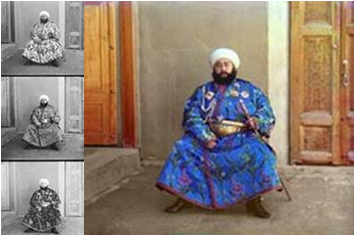
\includegraphics[width=0.65\linewidth]{example-Prokudin-Gorskii.png}
\caption{Example image from the Prokudin-Gorskii collection. On the left are the three images captured individually. On the right is a reconstructed color photograph. Note the colors are in B, G, R order from the top to bottom (and not R, G, B)!}
\end{figure}

The key step to compute the color image is to align the three photographs. Alas, since the camera moved between each shot, these channels are slightly displaced from each other. The simplest way is to keep one channel fixed say R, and align the G, B channels to it by searching over displacements in the range [-15, 15] both horizontally and vertically and pick the displacement that maximizes similarity between the channels. One such measure is the angle between vectors representing the pixels in each channel.

\subsection{Code}
Download the \cmd{p1.tar.gz} from the moodle page. Move them to your homework directory and extract the files (e.g. by typing \cmd{tar -xvf p1.tar.gz}). The code, data, and latex source files are in the \cmd{p1/code}, \cmd{p1/data}, and \cmd{p1/latex} folders respectively.

Before you start aligning the Prokudin-Gorskii images (in $\cmd{data/prokudin-gorskii}$), you will test your code on synthetic images which have been randomly shifted. Your code should correctly discover the inverse of the shift.

Run \cmd{evalAlignment} inside the code directory. This should produce the following output. Note the actual 'gt shift' might be different since it is randomly generated.
\begin{verbatim}
    Evaluating alignment ..
    1 balloon.jpeg
	   gt shift: ( 1,11) ( 4, 5)
	 pred shift: ( 0, 0) ( 0, 0)
    2 cat.jpg
	   gt shift: (-5, 5) (-6,-2)
	 pred shift: ( 0, 0) ( 0, 0)
     ...
\end{verbatim}
    
The code loads a set of images, randomly shifts the color channels and provides them as input to \cmd{alignChannels}. Your goal is to implement this function. A correct implementation should obtain the shifts that is the negative of the ground-truth shifts, i.e. the following output:

\begin{verbatim}
    Evaluating alignment ..
    1 balloon.jpeg
	   gt shift: ( 13, 11)  ( 4, 5)
	 pred shift: (-13,-11)  (-4,-5)
    2 cat.jpg
	   gt shift: (-5, 5) (-6,-2)
	 pred shift: ( 5,-5) ( 6, 2)
     ...
\end{verbatim}
    
Once you are done with that, run \cmd{alignProkudin}. This will call your function to align images from the Prokudin-Gorskii collection. The output is saved to the \cmd{outDir}. Note: if this directory does not exist, you will have to create it first. In your report, show all the aligned images as well as the shifts that were computed by your algorithm.

Tips: Look at functions \cmd{circshift()} and \cmd{padarray()} to deal with shifting images in Matlab. In Python, look for \cmd{np.roll} and \cmd{np.pad}.

\subsection{What to submit?}
To get full credit for this part you have to 
\begin{itemize}
\item include your implementation of \cmd{alignChannels},
\item verify that the \cmd{evalAlignment} correctly recovers the color image and shifts for the toy example, 
\item include the aligned color images from the output of \cmd{alignProkudin},
\emph{including} the computed shift vectors for each image.
\end{itemize}

\subsection{Extra credit}
Here are some ideas for extra credit.
\begin{itemize}
\item Shifting images can cause ugly boundary artifacts. Come up with of a way of avoiding this.
\item Searching over displacements can be slow. Think of a way of aligning them faster in a coarse-to-fine manner. For example, you may align the channels by resizing them to half the size and then refining the estimate. This can be done by multiple calls to your \cmd{alignChannels()} function.
\end{itemize}
If you do these, or any other, for extra credit make sure to include the code, description and any other details that you think are relevant for grading such as figures, run-time analysis, etc.

\newpage
\section{Color image demosaicing [30 points]}
Recall that in digital cameras the red, blue, and green sensors are interlaced in the Bayer pattern (Figure~\ref{fig:bayer}). The missing values are interpolated to obtain a full color image. For this part you will implement a simple interpolation algorithm called the \emph{nearest-neighbor} interpolation. The input to the algorithm is a single image im, a NxM array of numbers between 0 and 1. These are measurements in the format shown in Figure~\ref{fig:bayer}, i.e., top left \cmd{im(1,1)} is red, \cmd{im(1,2)} is green, \cmd{im(2,1)} is green, \cmd{im(2,2)} is blue, etc. Your goal is to create a single color image C from these measurements. Note that in Python/NumPy, those coordiantes are expressed as \cmd{im[0,0]}, \cmd{im[0,1]}, \cmd{im[1,0]}, \cmd{im[1,1]}.
\begin{figure}[h]
\centering
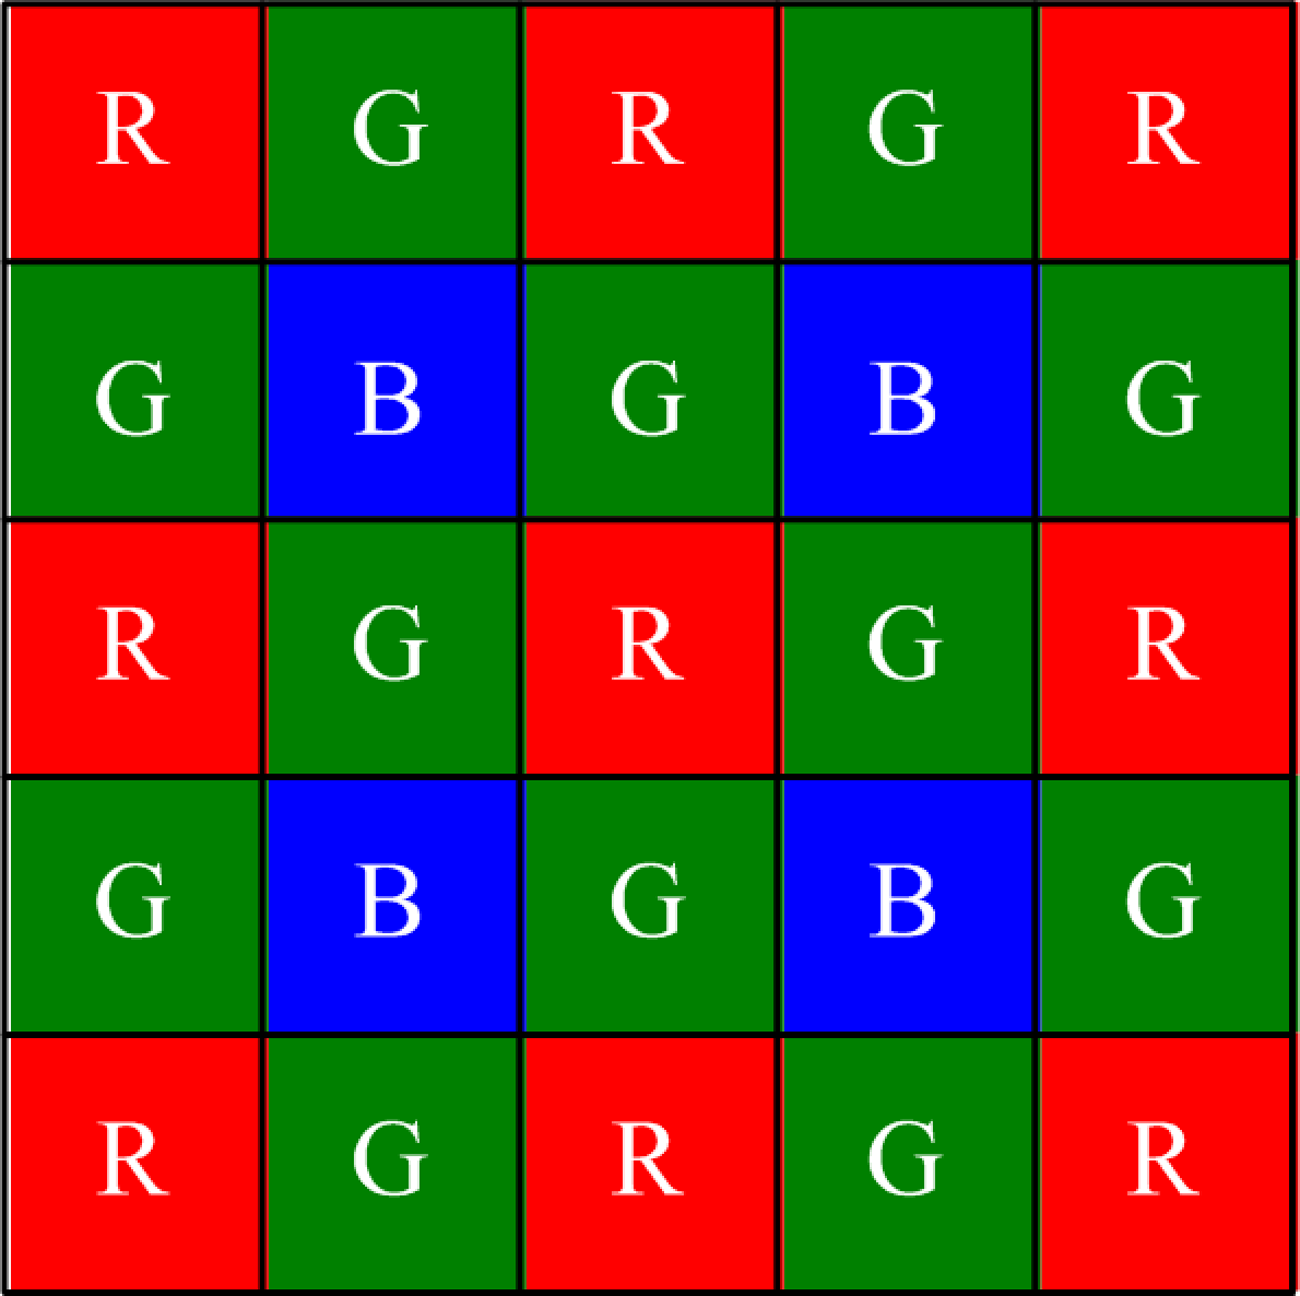
\includegraphics[width=0.2\linewidth]{bayer-pattern.png}
\caption{\label{fig:bayer} Bayer pattern}
\end{figure}

Your entry point for this part of the homework in \cmd{evalDemosaic}. The code loads images from the data directory (in $\cmd{data/demosaic}$), artificially mosaics them (\cmd{mosaicImage} file), and provides them as input to the demosaicing algorithm (\cmd{demosaicImage} file). By comparing the result with the input we can also compute the reconstruction error measured as the distance between the reconstructed image and the true image. This is what the algorithm reports. Once you have implemented the \cmd{mosaicImage} function run the \cmd{evalDemosaic} and you should see the output below.

Right now only the \cmd{demosaicImage(im, 'baseline')} is implemented which simply replaces all the missing values for a channel with the average value of that channel. You will implement the option \cmd{demosaicImage(im, 'nn')} which hopefully will obtain a significantly lower error and visually pleasing results. Right now it simply calls the baseline algorithm hence the two methods produce identical results.

\begin{verbatim}
--------------------------------------------
# 	 image             baseline   nn
--------------------------------------------
1 	 balloon.jpeg      0.179239 	 0.179239 
2 	 cat.jpg           0.099966 	 0.099966 
3 	 ip.jpg            0.231587 	 0.231587 
4 	 puppy.jpg         0.094093 	 0.094093 
5 	 squirrel.jpg      0.121964 	 0.121964 
6 	 pencils.jpg 	     0.183101 	 0.183101 
7 	 house.png         0.117667 	 0.117667 
8 	 light.png         0.097868 	 0.097868 
9 	 sails.png         0.074946 	 0.074946 
10  tree.jpeg         0.167812 	 0.167812 
--------------------------------------------
 	  average           0.136824 	 0.136824 
--------------------------------------------
\end{verbatim}
You will implement the two functions:
\begin{enumerate}
\item \points{10 points} Implement \cmd{mosaicImage(im)}. This function takes an image \cmd{im} with three color channels and returns an output \cmd{mosim} which has a single channel where the red, green, and blue pixels are copied according to the Bayer pattern shown in the figure. 
\item \points{20 points} Implement \cmd{demosaicImage(im, 'nn')}. This function takes the demosaiced image and reconstructs the three color channels. The `nn' option stands for \emph{nearest-neighbor} interpolation, i.e. you simply copy the value of the nearest available pixel. For example, each missing green pixel can copy the value  of the green pixel to its left (note that this doesn't work on the left boundary where you can copy from the top or bottom). This very simple method should produce reasonable results and substantially lower errors (around $0.025$ average error) when you run \cmd{evalDemosaic}
\end{enumerate}

\subsection{What to submit?}
To get full credit for this part you have to 
\begin{itemize}
\item include your implementation of \cmd{mosaicImage} and \cmd{demosaicImage},
\item include the output of \cmd{evalDemosaic}.
\end{itemize}

\subsection{Extra credit}
There are numerous other approaches for interpolation which you can read on the internet. You can use the ideas but do not copy the code (we can easily detect if you have simply copied the code from the web). You can implement this as other options \cmd{demosaicImage(im, `yourmethod')} and include the list of options in the \cmd{evalDemosaic} code. It is possible to get errors as low as $0.017$ without too much effort.
\end{document}
